\documentclass[12pt,a4paper]{article}

% Margins.
\setlength{\oddsidemargin}{0in}
\setlength{\evensidemargin}{0in}
\setlength{\headheight}{12pt}
\setlength{\headsep}{42pt}
\setlength{\topmargin}{-54pt}
\setlength{\textwidth}{6.5in}
\setlength{\textheight}{10in}

\usepackage{amsmath}
\usepackage{float}
\usepackage{graphicx}
\usepackage[hyphens]{url}
\usepackage{hyperref}	% Clickable links to figures, references and urls.
\usepackage{datetime}
\usepackage{longtable}
\usepackage{subfigure}

% Links direct to top of figures.
\usepackage[all]{hypcap}

% Drawing.
\usepackage{pgf}
\usepackage{tikz}

% Listings for formatting code.
\usepackage{listings}
\usepackage{textcomp}
% General options.+++
\lstset{breaklines=true, basicstyle=\small\ttfamily, tabsize=4, numbers=left, stepnumber=1, frame=single, showstringspaces=false, upquote=true}
% C++ specific high-lighting. Comments are 50/50 shades of green/black and strings coloured with 60/40 red/black mixture.
\lstset{language=[ISO]C++, commentstyle=\color{green!50!black}, keywordstyle=\color{blue}, stringstyle=\color{red!60!black}}

%opening
\title{\vspace{-3cm}Physics for Engineers\\Class 20\\Electric Field of Point Charges: Problems}
\author{Attique Dawood}
\date{October 02, 2013\\[0.2cm] Last Modified: \today, \currenttime}
\begin{document}
\maketitle
\section{Announcements}
\begin{itemize}
\item None.
\end{itemize}
\section{Revision}
\begin{itemize}
\item Electric field of uniform ring of charge.
\item Electric field of uniform disk of charge.
\end{itemize}
\section{Exercises}
\noindent\textbf{Question 1 \cite[Problem 10, page 731]{Serway}:} Two small beads having positive charges $3q$ and $q$ are fixed at the opposite ends of a horizontal, insulating rod, extending from the origin to the point $x=d$. As shown in figure \ref{Equilibrium}, a third small charged bead is free to slide on the rod. At what position is the third bead in equilibrium?
\begin{figure}[H]
\centering
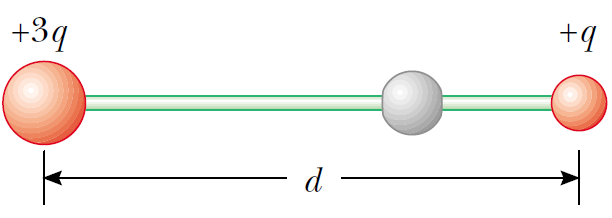
\includegraphics[scale=0.45]{FigureP23-10.png}
\caption{Equilibrium of charge.}
\label{Equilibrium}
\end{figure}
\noindent\textbf{Question 2 \cite[Problem 15, page 731]{Serway}:} In figure \ref{Electric-field-zero}, determine the point (other than infinity) at which the electric field is zero.
\begin{figure}[H]
\centering
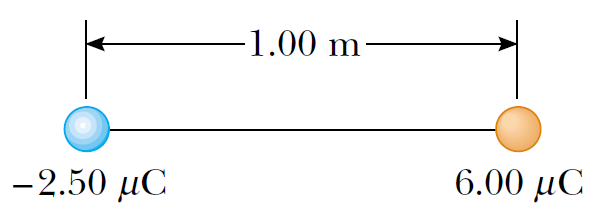
\includegraphics[scale=0.45]{FigureP23-15.png}
\caption{Finding location of zero field.}
\label{Electric-field-zero}
\end{figure}
\newpage
\noindent\textbf{Question 3 \cite[Problem 21, page 732]{Serway}:} Four point charges are at the corners of a square of side $a$ as shown in figure \ref{E-field-at-q}.
\begin{itemize}
\item[a.] Determine the magnitude and direction of the electric field at the location of charge $q$.
\item[b.] What is the resultant force on $q$?
\end{itemize}
\begin{figure}[H]
\centering
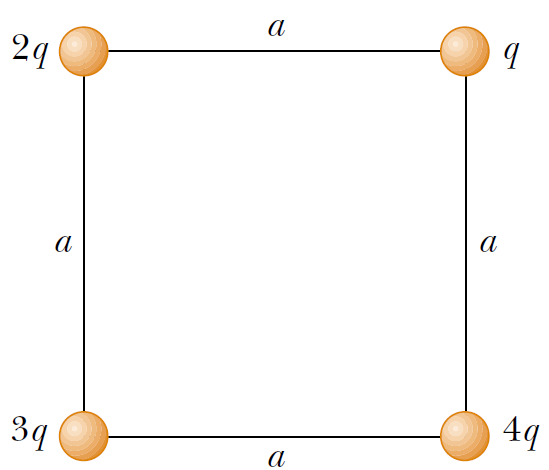
\includegraphics[scale=0.45]{FigureP23-21.png}
\caption{Force on charge $q$.}
\label{E-field-at-q}
\end{figure}
%\nocite{*}
\bibliographystyle{plain}
\bibliography{PhysicsRef}
\end{document}
